\documentclass[11pt]{beamer}
\graphicspath{{img/}{./}}
\usepackage[french]{babel}
\usepackage{graphicx}
\usepackage{ulem} %Pour biffer du texte \sout{texte barré}
\usepackage{xcolor} 
\usepackage{tabularx}
\usepackage{parallel}
%\usepackage[babelshorthands]{polyglossia}
\usepackage{ragged2e} 


%Allignemebnt droite/gauche
\usepackage{polyglossia}
%\usepackage[babelshorthands]{polyglossia} %[babelshorthands] permet d'avoir les guillemets allemands avec le code "`toto"' et les guillemets français avec le code "<tata">


\usepackage{multirow} 
\setmainlanguage{english}
\usepackage[autostyle]{csquotes}
\MakeOuterQuote{"}
\DeclareQuoteStyle{english}%
    {\textquotedblleft}
    [\textquotedblleft]
    {\textquotedblright}
        [0.05em]
    {\textquoteleft}
    [\textquoteleft]
    {\textquoteright}
% \DeclareQuoteStyle[quotes]{french}
%   {\mkfrenchopenquote{«}}
%   {\mkfrenchclosequote{\nobreakspace»}}
%   {\textquotedblleft}
%   {\textquotedblright}
% \DeclareQuoteStyle[quotes*]{french}
%   {\mkfrenchopenquote{«}}
%   {\mkfrenchclosequote{\nobreakspace»}}
%   {\mkfrenchopenquote{\textquotedblleft}}
%   {\mkfrenchclosequote{\textquotedblright}}
% \DeclareQuoteStyle[guillemets]{french}
%   [\initfrenchquotes]
%   {\mkfrenchopenquote{«}}
%   [\mkfrenchopenquote{«}]
%   {\mkfrenchclosequote{\nobreakspace»}}
%   {\mkfrenchopenquote{«}}
%   [\mkfrenchopenquote{«}]
%   {\mkfrenchclosequote{\nobreakspace»}}
% \DeclareQuoteStyle[guillemets*]{french}
%   [\initfrenchquotes]
%   {\mkfrenchopenquote{«}}
%   [\mkfrenchopenquote{\nobreakspace»}]
%   {\mkfrenchclosequote{\nobreakspace»}}
%   {\mkfrenchopenquote{«}}
%   [\mkfrenchopenquote{\nobreakspace»}]
%   {\mkfrenchclosequote{\nobreakspace»}}




\setotherlanguage{greek}
\newfontfamily\greekfont[Script=Greek]{Linux Libertine O}
\newfontfamily\greekfontsf[Script=Greek]{Linux Libertine O}
\setotherlanguage{hebrew}
\newfontfamily{\hebrewfont}[Script=Hebrew, Path=./fonts/]{SBL_Hbrw.ttf}
\newfontfamily{\hebrewfontsf}[Script=Hebrew]{Miriam CLM}
\newfontfamily{\hebrewfonttt}[Script=Hebrew]{Miriam Mono CLM}
\setotherlanguage{syriac}
\newfontfamily\syriacfont[Script=Syriac, Path=./fonts/]{EstrangeloEdessa.ttf}

\usepackage{booktabs} % Allows the use of \toprule, \midrule and \bottomrule for better rules in tables
%% Allow the use of tcolorbox
\usepackage[skins]{tcolorbox}
%\usetheme{default}
%\usetheme{AnnArbor}
%\usetheme{Antibes}
%\usetheme{Bergen}
%\usetheme{Berkeley}
%\usetheme{Berlin}
%\usetheme{Boadilla}
%\usetheme{CambridgeUS}
%\usetheme{Copenhagen}
%\usetheme{Darmstadt}
%\usetheme{Dresden}
%\usetheme{Frankfurt}
%\usetheme{Goettingen}
%\usetheme{Hannover}
%\usetheme{Ilmenau}
\usetheme{JuanLesPins}
%\usetheme{Luebeck}
%\usetheme{Madrid}
%\usetheme{Malmoe}
%\usetheme{Marburg}
%\usetheme{Montpellier}
%\usetheme{PaloAlto}
%\usetheme{Pittsburgh}
%\usetheme{Rochester}
%\usetheme{Singapore}
%\usetheme{Szeged}
%\usetheme{Warsaw}

%----------------------------------------------------------------------------------------
%	SELECT COLOR THEME
%----------------------------------------------------------------------------------------

% Beamer comes with a number of color themes that can be applied to any layout theme to change its colors. Uncomment each of these in turn to see how they change the colors of your selected layout theme.

%\usecolortheme{albatross}
%\usecolortheme{beaver}
%\usecolortheme{beetle}
%\usecolortheme{crane}
%\usecolortheme{dolphin}
%\usecolortheme{dove}
%\usecolortheme{fly}
%\usecolortheme{lily}
%\usecolortheme{monarca}
%\usecolortheme{seagull}
%\usecolortheme{seahorse}
%\usecolortheme{spruce}
%\usecolortheme{whale}
%\usecolortheme{wolverine}

%----------------------------------------------------------------------------------------
%	SELECT FONT THEME & FONTS
%----------------------------------------------------------------------------------------
\setmainfont{cochineal}
% Beamer comes with several font themes to easily change the fonts used in various parts of the presentation. Review the comments beside each one to decide if you would like to use it. Note that additional options can be specified for several of these font themes, consult the beamer documentation for more information.

%\usefonttheme{default} % Typeset using the default sans serif font
\usefonttheme{serif} % Typeset using the default serif font (make sure a sans font isn't being set as the default font if you use this option!)
%\usefonttheme{structurebold} % Typeset important structure text (titles, headlines, footlines, sidebar, etc) in bold
%\usefonttheme{structureitalicserif} % Typeset important structure text (titles, headlines, footlines, sidebar, etc) in italic serif
%\usefonttheme{structuresmallcapsserif} % Typeset important structure text (titles, headlines, footlines, sidebar, etc) in small caps serif

%------------------------------------------------

%\usepackage{mathptmx} % Use the Times font for serif text
%\usepackage{palatino} % Use the Palatino font for serif text


%\usepackage{helvet} % Use the Helvetica font for sans serif text
%\usepackage[default]{opensans} % Use the Open Sans font for sans serif text
%\usepackage[default]{FiraSans} % Use the Fira Sans font for sans serif text
%\usepackage[default]{lato} % Use the Lato font for sans serif text

%----------------------------------------------------------------------------------------
%	SELECT INNER THEME
%----------------------------------------------------------------------------------------

% Inner themes change the styling of internal slide elements, for example: bullet points, blocks, bibliography entries, title pages, theorems, etc. Uncomment each theme in turn to see what changes it makes to your presentation.

%\useinnertheme{default}
%\useinnertheme{circles}
\useinnertheme{rectangles}
%\useinnertheme{rounded}
%\useinnertheme{inmargin}

%----------------------------------------------------------------------------------------
%	SELECT OUTER THEME
%----------------------------------------------------------------------------------------

% Outer themes change the overall layout of slides, such as: header and footer lines, sidebars and slide titles. Uncomment each theme in turn to see what changes it makes to your presentation.

%\useoutertheme{default}
%\useoutertheme{infolines}
%\useoutertheme{miniframes}
%\useoutertheme{smoothbars}
%\useoutertheme{sidebar}
%\useoutertheme{split}
%\useoutertheme{shadow}
%\useoutertheme{tree}
%\useoutertheme{smoothtree}

%\setbeamertemplate{footline} % Uncomment this line to remove the footer line in all slides
%\setbeamertemplate{footline}[page number] % Uncomment this line to replace the footer line in all slides with a simple slide count

%\setbeamertemplate{navigation symbols}{} % Uncomment this line to remove the navigation symbols from the bottom of all slides
\usepackage[style=sbl]{biblatex}


\DeclareSourcemap{
  \maps[datatype=bibtex]{
    \map{
      \step[fieldset=doi, null]
      \step[fieldset=language, null]
      \step[fieldset=issn, null]{}
      \step[fieldset=url, null]{}
      \step[fieldset=isbn, null]{}
      \step[fieldset=eprint, null]{}
    }
  }
}

\addbibresource{references.bib}
%\defbibheading{bibempty}{}

%----------
% Define sectioning
\AtBeginSection[]{
  \begin{frame}
  \vfill
  \centering
  \begin{beamercolorbox}[sep=8pt,center,shadow=true,rounded=true]{title}
    \usebeamerfont{title}\insertsectionhead\par%
  \end{beamercolorbox}
  \vfill
  \end{frame}
}

%-----------

%----------------------------------------------------------------------------------------
%	PRESENTATION INFORMATION
%----------------------------------------------------------------------------------------


\title{Introduction à la critique textuelle}
\author[Frédérique Michèle Rey, Sophie Robert-Hayek]{Frédérique Michèle Rey \& Sophie Robert-Hayek}


\institute[UL]{Université de Lorraine } %\smallskip \textit{frederique.rey@univ-lorraine.fr / sophie.robert@univ-lorraine.fr}}

\date{}
\usepackage[table]{xcolor}
\usepackage[dvipsnames]{xcolor}
\usepackage{forest}
\usepackage{tikz-qtree}
\usepackage[font=scriptsize]{caption}
\begin{document}

\section{1. Petite histoire de la philologie}

\section{Qu'est-ce que la critique textuelle ?}

\begin{frame}{Définition de Paul Maas}
    \begin{figure}
        \centering
        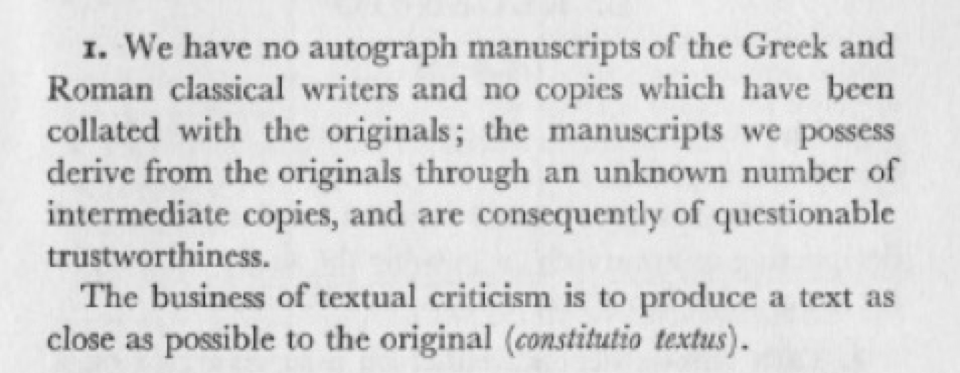
\includegraphics[width=1\linewidth]{img/maas_definition.png}
    \end{figure}
    \tiny{\footnotesize{\fullcite[1]{maas_textkritik_1960}}}
\end{frame}

\section{La vérité de l'auteur}
\begin{frame}{La vérité de l'auteur : les éditions Lachmaniennes}
    \begin{minipage}{.4\textwidth}
        \begin{figure}
            \centering
            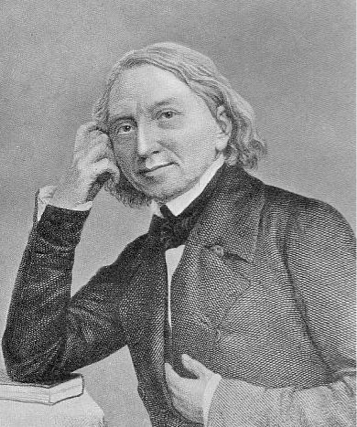
\includegraphics[width=1\linewidth]{img/lachman.png}
            \caption{Karl Lachman (1793-1851)}
        \end{figure} 
    \end{minipage}%
    \hfill
    \begin{minipage}{.6\textwidth}
         \begin{itemize}
            \item Editions de type lachmanienne
            \item Modèle reconstructionniste
            \item Fidélité à l'auteur
            \item Utilisation d'un \textit{stemma codicum} pour reconstruire l'archétype, ou le \textit{Urtext} ("original")
        \end{itemize}
    \end{minipage}
\end{frame}

\begin{frame}{La vérité de l'auteur : les éditions Lachmaniennes}
    \begin{minipage}{.4\textwidth}
        \begin{figure}
            \centering
            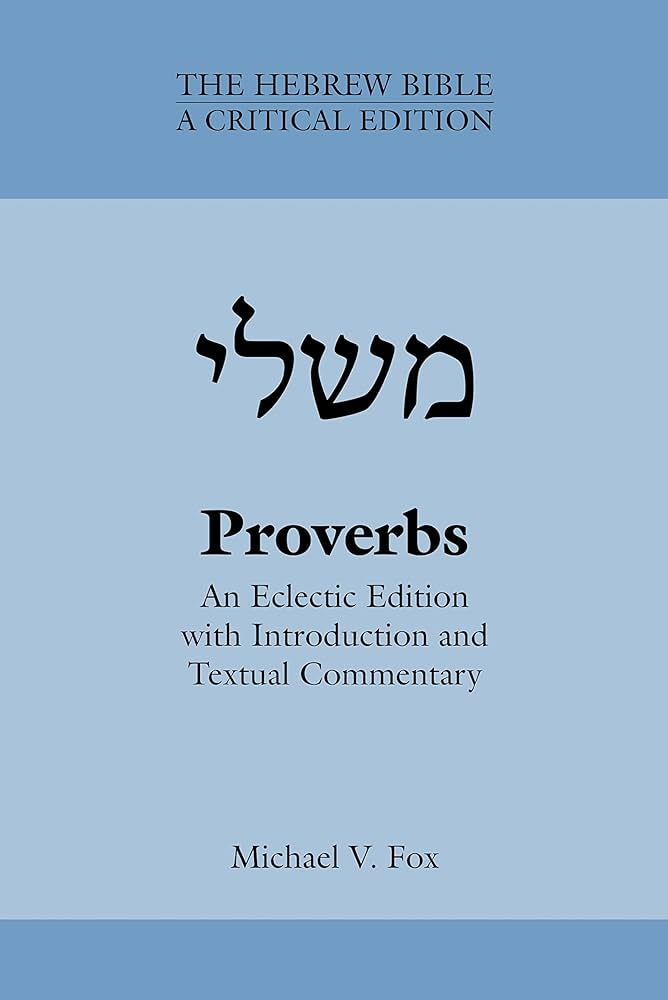
\includegraphics[width=1\linewidth]{img/fox_cover.jpg}
        \end{figure} 
    \end{minipage}%
    \hfill
    \begin{minipage}{.5\textwidth}
        \begin{block}{Dans les études bibliques}
            \begin{itemize}
                \item Paul De Lagarde (1827-1891)\\
                        \footnotesize{\fullcite[]{lagarde_anmerkung_1884}}
                \item The Hebrew Bible a Critical Edition Project (dir. Ron Hendel, Berkeley)
                \item Nestle-Aland, \textit{Novum Testamentum Graece}
            \end{itemize}   
        \end{block}
    \end{minipage}
\end{frame}

\begin{frame}{Définitions}
    \begin{definition}
        On appelle \textbf{\textit{Stemma Codicum}}, l'arbre généalogique des manuscrits d'une tradition textuelle.
    \end{definition}
    \pause
    \begin{definition}
        On appelle \textbf{archetype}, la reconstruction hypothétique d'un texte au sommet de l'arbre généalogique qui permette d'expliquer les formes textuelles de l'ensemble de ses descendants.
    \end{definition}
    \pause
    \begin{definition}
        La définition de l'\textbf{original} (\textit{Urtext}) est l'une des questions les plus floue de la critique textuelle: ce que l'auteur a écrit? L'autographe? L'autographe corrigé? Ce que l'auteur aurait voulu écrire (l'intention de l'auteur)? La première édition d'un texte? etc.
    \end{definition}
\end{frame}


\begin{frame}{Exercice : la transmission textuelle trouble d'Harry Potter}
    \begin{minipage}{.45\textwidth}
        \begin{block}{}
            [A] Mr and Mrs {Potter},\\ of number {pour}, Privet Drive
        \end{block}
        \begin{block}{}
            [B] Mr and Mrs Dursley,\\ of number four, Private Drive
        \end{block}
        \begin{block}{}
            [C] {Mr Dursley},\\ of number four, {Private} Drive
        \end{block}

    \end{minipage}
    \hfill
    \begin{minipage}{.45\textwidth}
         \begin{block}{}
            [D] Mr and Mrs Dursley,\\ of number four, Privet Drive 
        \end{block}
        \begin{block}{}
            [E] {Mrs and Mr} Dursley,\\ of number {pour}, Privet Drive
        \end{block}
        \begin{block}{}
            [F] Mr and Mrs Dursley,\\ of number pour, Privet Drive
        \end{block}     
    \end{minipage}
\end{frame}

\begin{frame}{Solution : la transmission textuelle trouble d'Harry Potter}
\scriptsize{
    \begin{forest} for tree={align=center, edge path={\noexpand\path[\forestoption{edge}] (\forestOve{\forestove{@parent}}{name}.parent anchor) -- +(0,-20pt)-| (\forestove{name}.child anchor)\forestoption{edge label};}}
        [{[D] Mr and Mrs Dursley,\\ of number four, Privet Drive}
            [{[F] Mr and Mrs Dursley,\\ of number \textcolor{BrickRed}{pour}, Privet Drive}
                [{[A] Mr and Mrs \textcolor{Orange}{Potter},\\ of number \textcolor{BrickRed}{pour}, Privet Drive}]
                [{[E] \textcolor{RoyalBlue}{Mrs and Mr} Dursley,\\ of number \textcolor{BrickRed}{pour}, Privet Drive}]
            ]
            [{[B] Mr and Mrs Dursley,\\ of number four, \textcolor{violet}{Private} Drive}
                [{[C] \textcolor{Green}{Mr Dursley},\\ of number four, \textcolor{violet}{Private} Drive}]
            ]
        ]
    \end{forest}
}
\end{frame}

\begin{frame}{Qu'est-ce que la stemmatologie ?}
    \begin{minipage}{.4\textwidth}
        \begin{figure}
            \centering
            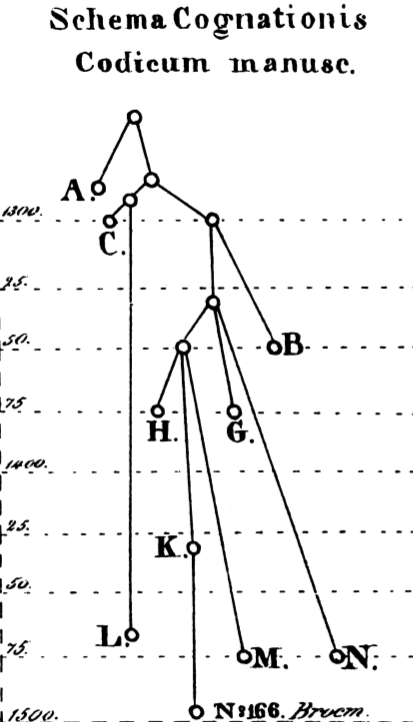
\includegraphics[width=0.7\linewidth]{img/stemmaschlyter.png}
            \caption{Stemma codicum de Schlyter (1827)}
        \end{figure} 
    \end{minipage}
    \hfill
    \begin{minipage}{.55\textwidth}
        \small{
        \begin{alertblock}{Stemmatologie}
            \textbf{La stemmatologie} est la science qui vise à reconstruire l'arbre généalogique (stemma) des différents manuscrits d'un texte donné:
            \begin{itemize}
                \item Pour \og reconstruire \fg un archétype (perspective reconstructionniste);
                \item Pour comprendre la transmission d'un texte à travers les siècles.
            \end{itemize}
        \end{alertblock}
        \vspace{.5cm}
        La stemmatologie est une branche de la critique textuelle.
        }
    \end{minipage}
\end{frame}

\begin{frame}{Paul Maas, \textit{Textkritik} (1927)}
    \begin{minipage}{.3\textwidth}
        \begin{figure}
            \centering
            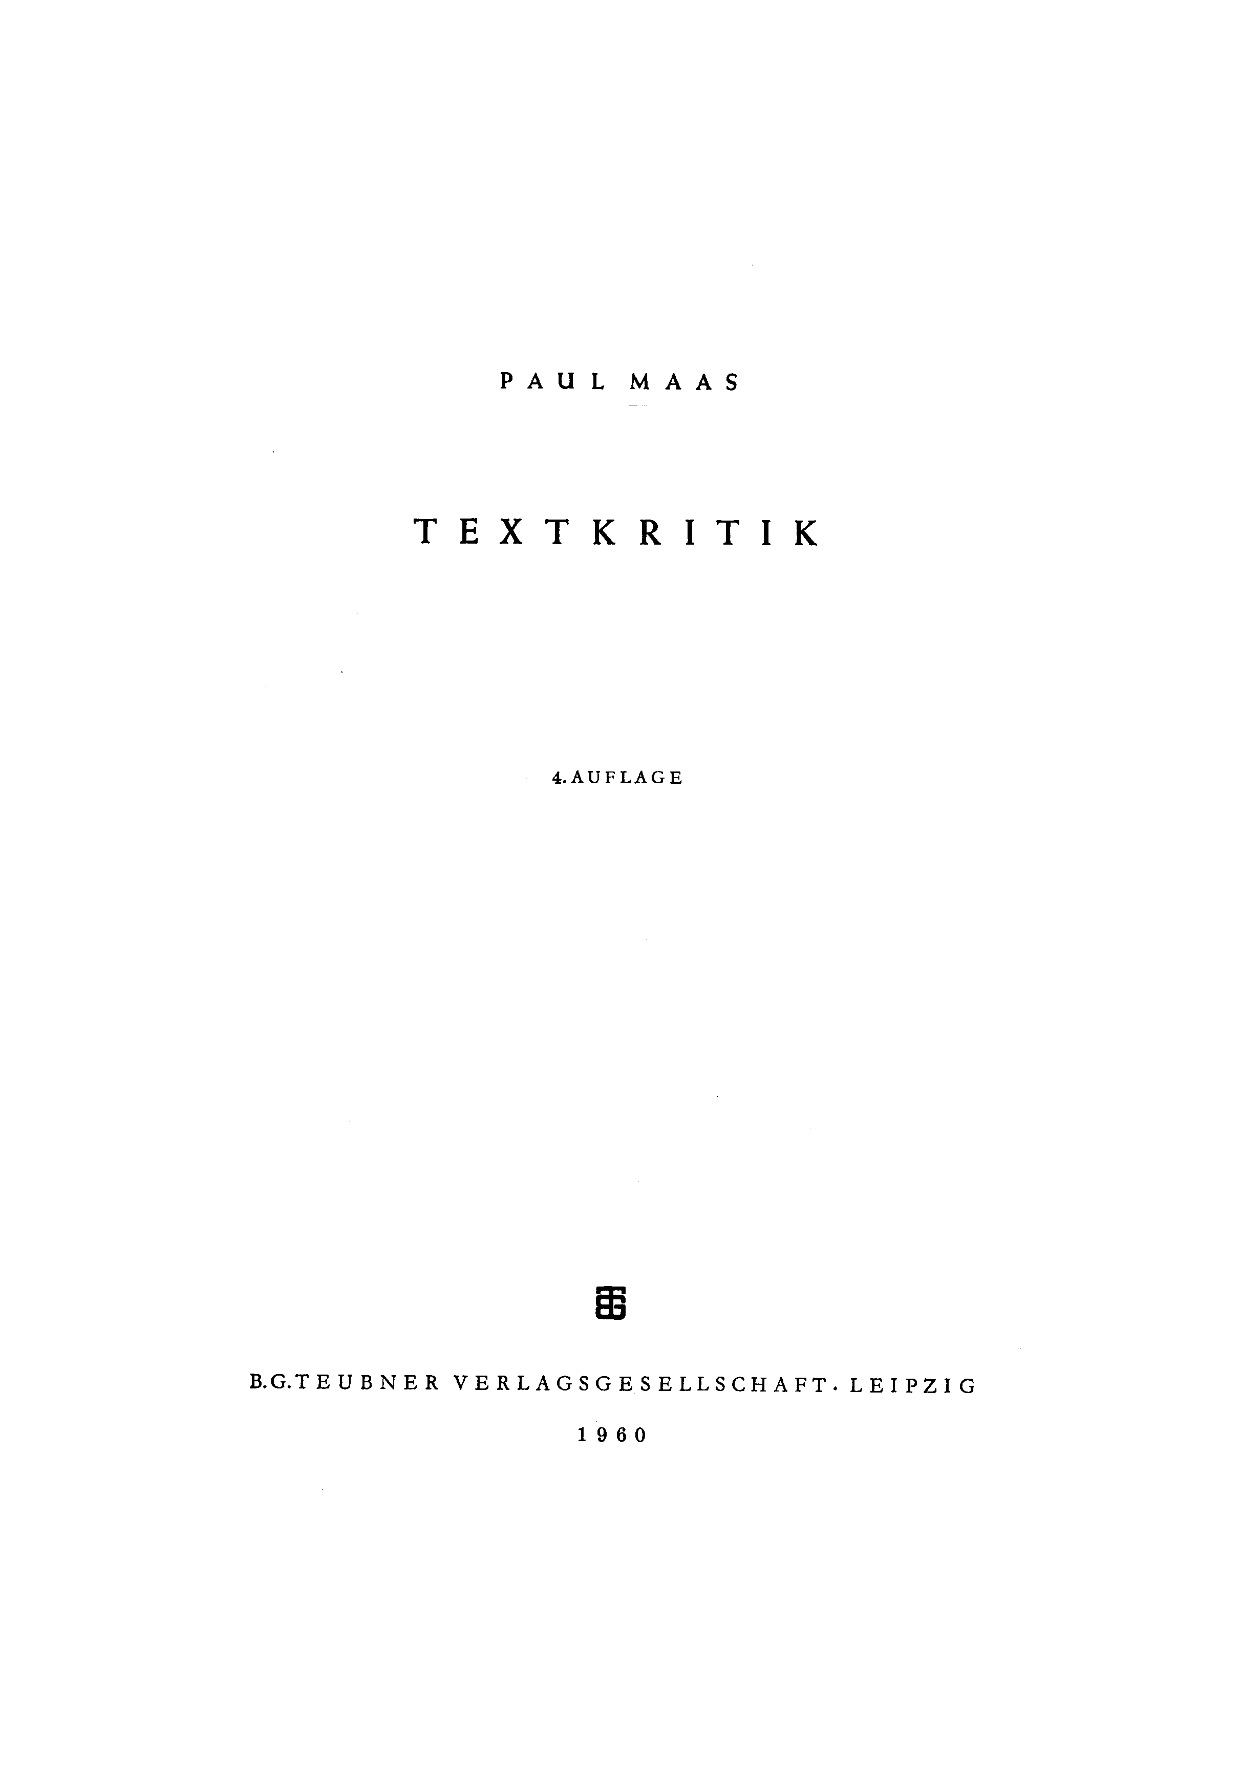
\includegraphics[width=1\linewidth]{img/maas.png}
        \end{figure} 
    \end{minipage}%
    \hfill
    \begin{minipage}{.7\textwidth}
        \small{
         \begin{itemize}
            \item Si deux manuscrits présentent une erreur \textbf{monogénétique} par rapport à un troisième manuscrit alors ces deux manuscrits appartiennent à la même ligne de transmission textuelle. Dans ce cas, on parlera d'\textbf{erreurs conjonctives}.
            \item Inversement, si deux manuscrits présentent des erreurs indépendantes, alors ces deux manuscrits n'appartiennent pas à la même ligne de transmission du texte ; dans ce cas, on parlera d'\textbf{erreurs séparatives}.
        \end{itemize}
        }
    \end{minipage}
\end{frame}

\begin{frame}{La transmission : un processus dégénératif}
\begin{block}{}
    Dans le modèle lachmanien, le processus de transmission est \textbf{décrit} comme un processus \textbf{dégénératifs}. Les scribes commettent des erreurs et ce sont ses \textbf{erreurs} qui permettent aux textualistes de remonter l'arbre jusqu'à l'archétype. Au fil du temps et des transmissions, le texte s'\textbf{altère}, se \textbf{dégrade}.\\

    Le concept d'original ou d'archétype a un côté très romantique. C'est la perfection perdue du texte qu'il faut retrouver. Le paradis perdu du texte.
\end{block}
    
\end{frame}

\section{La vérité du témoin}

\begin{frame}{La vérité du témoin : les éditions bédiéristes}
\begin{minipage}{.45\textwidth}
\begin{block}{Éditions bédiéristes}
\begin{itemize}
    \item Éditer un seul manuscrit (le meilleur ?) et indiquer les variantes dans une apparat
    \item Une fidélité au scribe
    \item Une fidélité au document
\end{itemize}
\end{block}
\end{minipage}
\hfill
\begin{minipage}{.5\textwidth}
    \begin{figure}
    \centering
    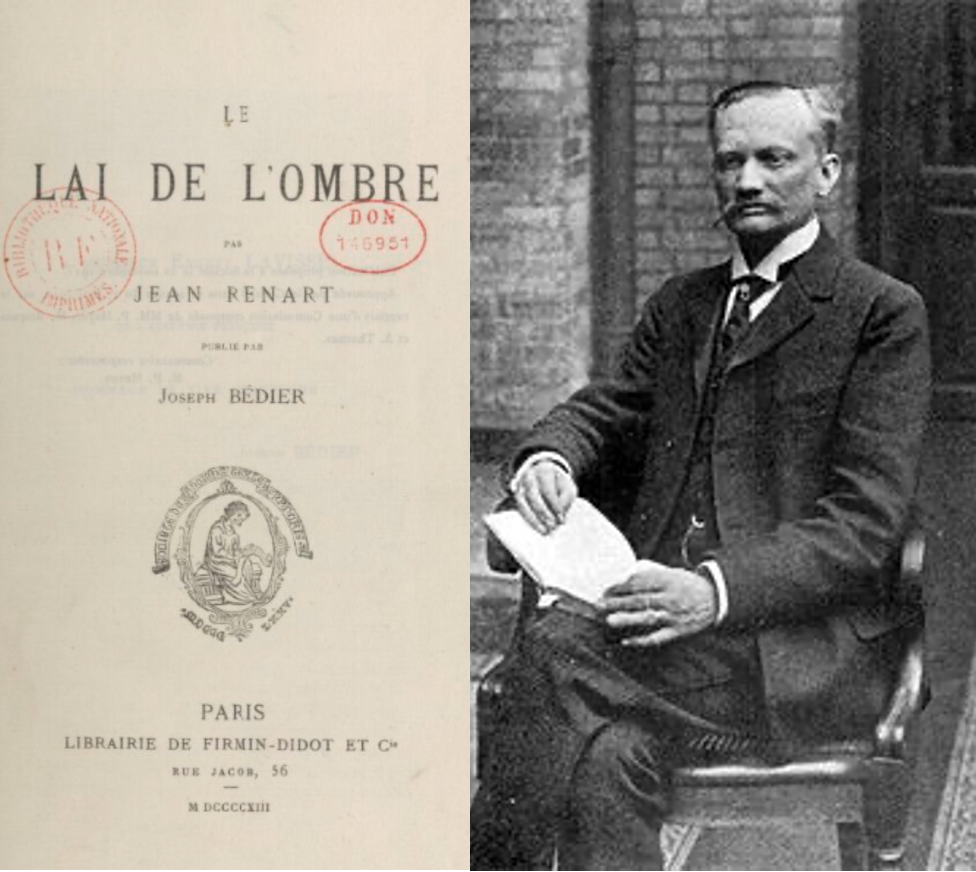
\includegraphics[width=1\linewidth]{img/bedier.png}
    \caption{Joseph Bédier (1864-1938)}
    \end{figure} 
\end{minipage}
\end{frame}

\begin{frame}{La vérité du témoin : les éditions bédiéristes}
\begin{minipage}{.45\textwidth}
\begin{block}{Éditions bédiéristes}
\begin{itemize}
    \item Éditer un seul manuscrit (le meilleur ?) et indiquer les variantes dans une apparat
    \item Une fidélité au scribe
    \item Une fidélité au document
\end{itemize}
\end{block}
\end{minipage}
\hfill
\begin{minipage}{.5\textwidth}
    \begin{figure}
    \centering
    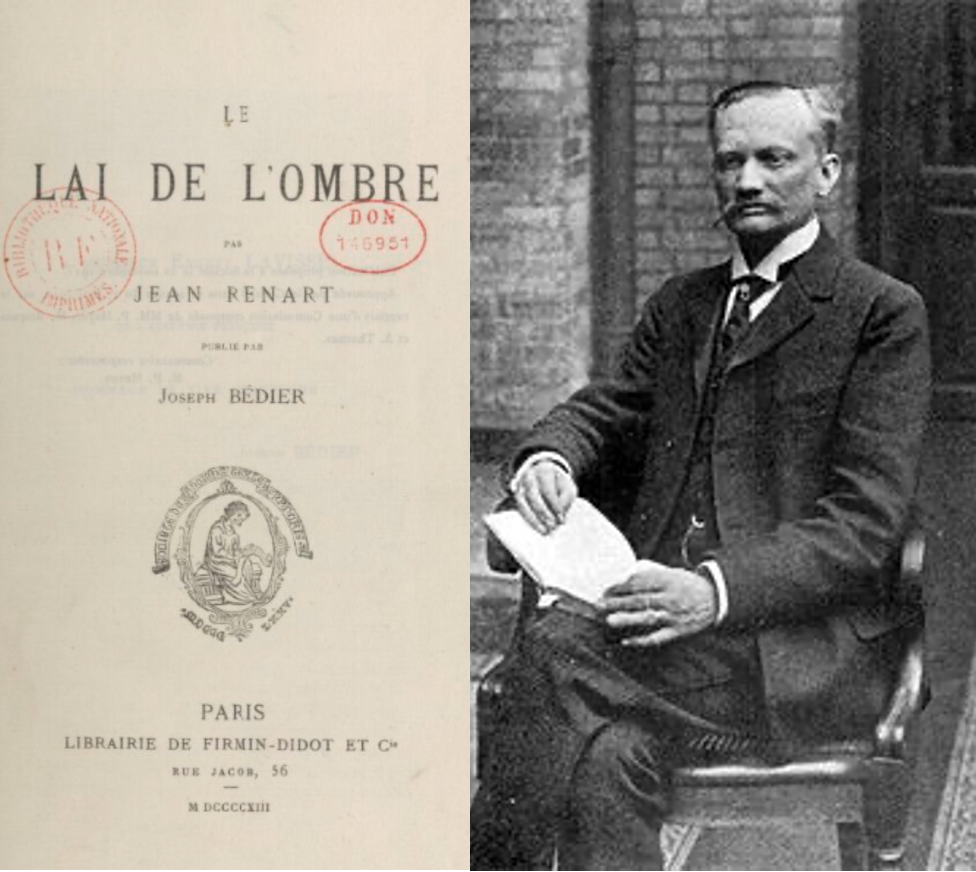
\includegraphics[width=1\linewidth]{img/bedier.png}
    \caption{Joseph Bédier (1864-1938)}
    \end{figure} 
\end{minipage}
\end{frame}

\begin{frame}{La vérité du témoin : les éditions bédiéristes}
\begin{minipage}{.45\textwidth}
\begin{block}{Dans les études bibliques}
\begin{itemize}
        \item Plusieurs stemma possibles
        \item Problème des stemmas bifides
        \item Travailler sur ce que l'on a (le manuscrit) plutôt que sur ce qu'on voudrait avoir (l'archétype)
\end{itemize}
\end{block}
\end{minipage}
\hfill
\begin{minipage}{.5\textwidth}
    \begin{figure}
    \centering
    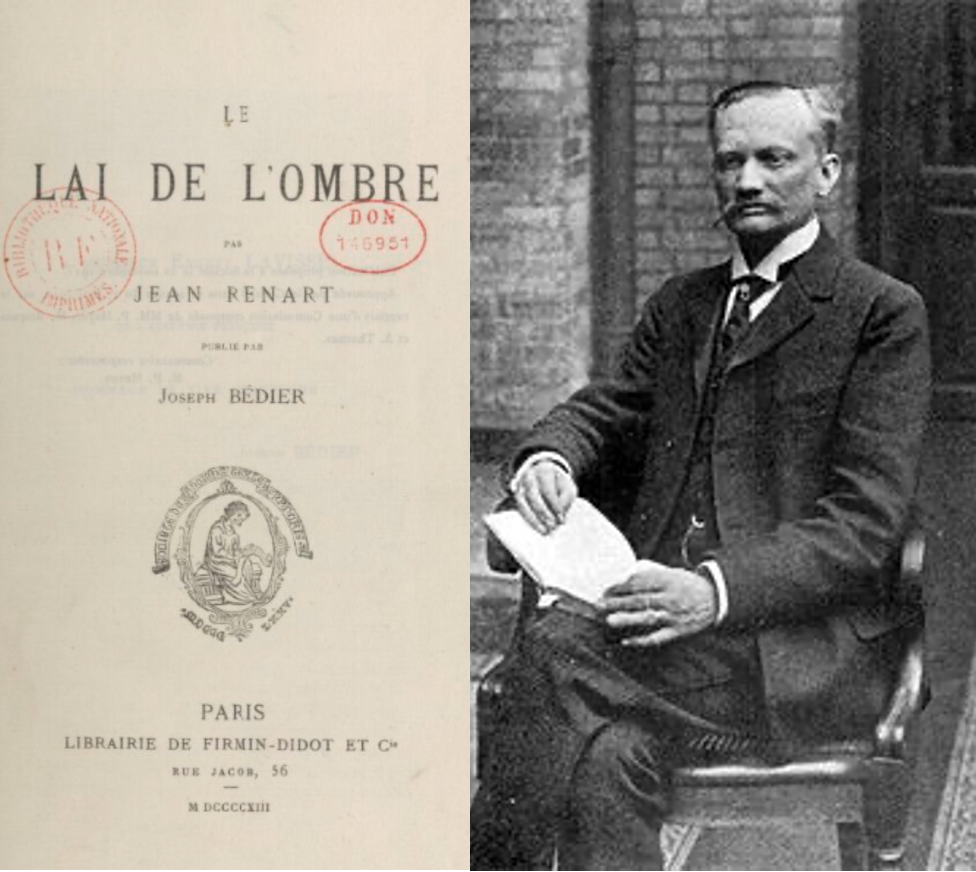
\includegraphics[width=1\linewidth]{img/bedier.png}
    \caption{Joseph Bédier (1864-1938)}
    \end{figure} 
\end{minipage}
\end{frame}


\begin{frame}{La vérité du témoin : les éditions bédiéristes}
\begin{exampleblock}{}
    Aussi la méthode d’édition la plus recommandable est-elle peut-être, en dernière analyse, celle que régit un esprit de défiance de soi, de prudence, d’extrême "conservatisme", un énergique vouloir, porté jusqu’au parti pris, d’ouvrir aux scribes le plus large crédit et de ne toucher au texte d’un manuscrit que l’on imprime qu’en cas d’extrême et presque évidente nécessité: toutes les corrections conjecturales devraient être reléguées en des appendices. « Une telle méthode d’édition, a écrit dom Quentin, risque d’être bien dommageable à la critique textuelle ». Peut-être ; mais c’est, de toutes les méthodes connues, celle qui risque le moins d’être dommageable aux textes.
\end{exampleblock}
\footnotesize{\fullcite[356]{bedier_tradition_1928}}
\end{frame}

\begin{frame}{La vérité du témoin : les éditions bédiéristes}
\begin{minipage}{.45\textwidth}
\begin{block}{Dans les études bibliques}
\begin{itemize}
        \item Paul Kahle (1875-1964)
        \item La \textit{Biblia Hebraica Stuttgartensia}
        \item La \textit{Biblia Hebraica Quinta}
        \item The Hebrew University Bible Project
\end{itemize}
\end{block}
\end{minipage}
\hfill
\begin{minipage}{.5\textwidth}
    \begin{figure}
    \centering
    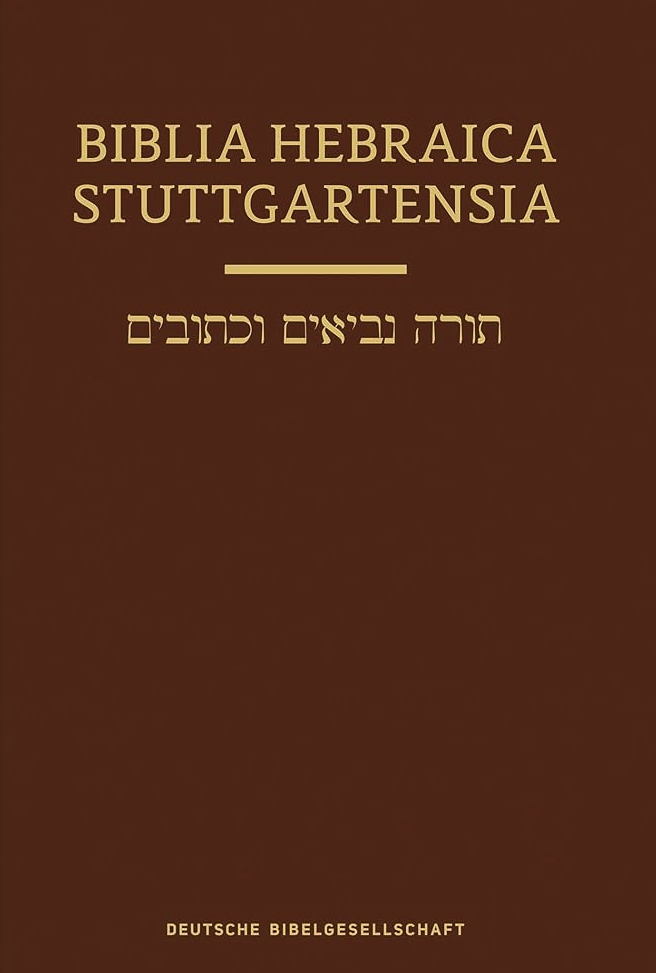
\includegraphics[width=1\linewidth]{img/bhs_cover.png}
    \end{figure} 
\end{minipage}
\end{frame}

\begin{frame}{Giorgio Pasquali, \textit{Storia della Tradizione e Critica del Testo}}
\begin{minipage}{.4\textwidth}
    \begin{figure}
    \centering
    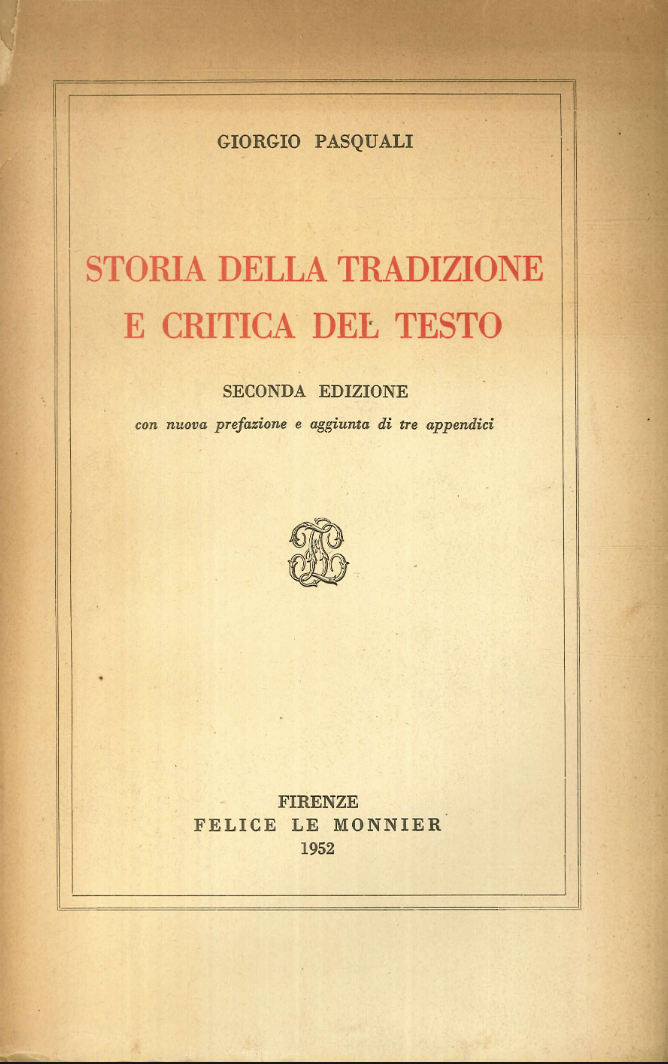
\includegraphics[width=1\linewidth]{img/pasquali.png}
    \end{figure} 
    \end{minipage}%
    \hfill
\begin{minipage}{.6\textwidth}
    \begin{block}{Une critique de Paul Maas}
     \begin{itemize}
        \item L'histoire de la tradition
        \item Non déterioration des traditions
        \item Les variantes d'auteurs
        \item Les archétypes multiples
        \item La contamination (transmission horizontale)

    \end{itemize}
    \end{block}
    \end{minipage}
    
\end{frame}



\begin{frame}{La \textit{New Philology}}
    \begin{minipage}{.45\textwidth}
        \begin{figure}
            \centering
            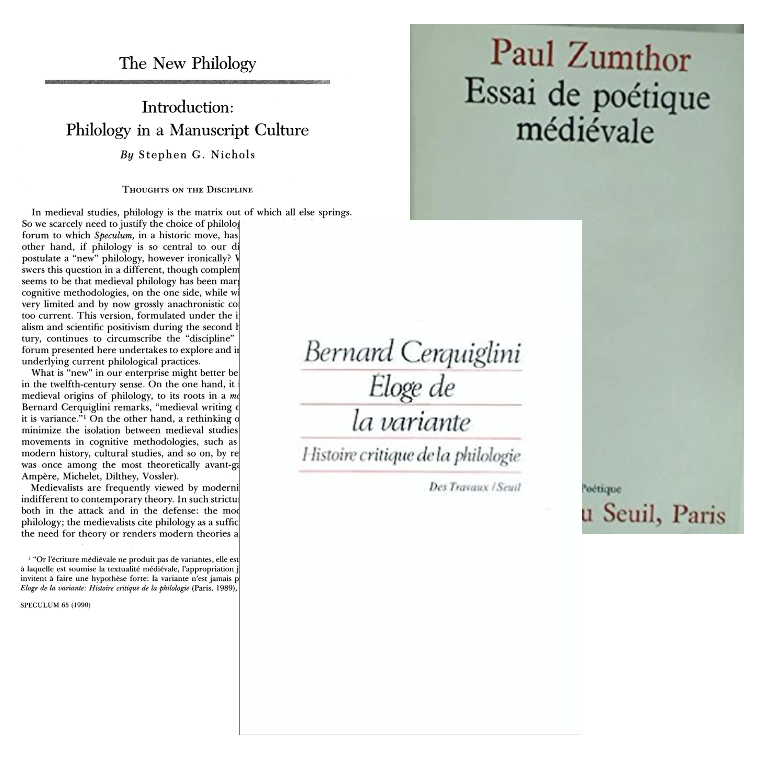
\includegraphics[width=1\linewidth]{img/new_philology.png}
            \caption{Bernard Cerquiglini, \textit{Éloge de la variante. Histoire critique de la philologie, 1989}}
        \end{figure}
    \end{minipage}%
    \hfill
    \begin{minipage}{.45\textwidth}
        \begin{block}{La "Nouvelle Philologie"}   
            \begin{itemize}
                \item Le manuscrit
                \item Sa matérialité
                \item Son contexte historique
                \item Le scribe
                \item La variance
                \item La question de l'auteur
                \item La question du texte
                \item  Ex. B. Cerquiglini
            \end{itemize}       
        \end{block}
    \end{minipage}


\end{frame}

\begin{frame}{L'histoire des transformations textuelles}

\begin{minipage}{.45\textwidth}


    \begin{figure}
        \centering
        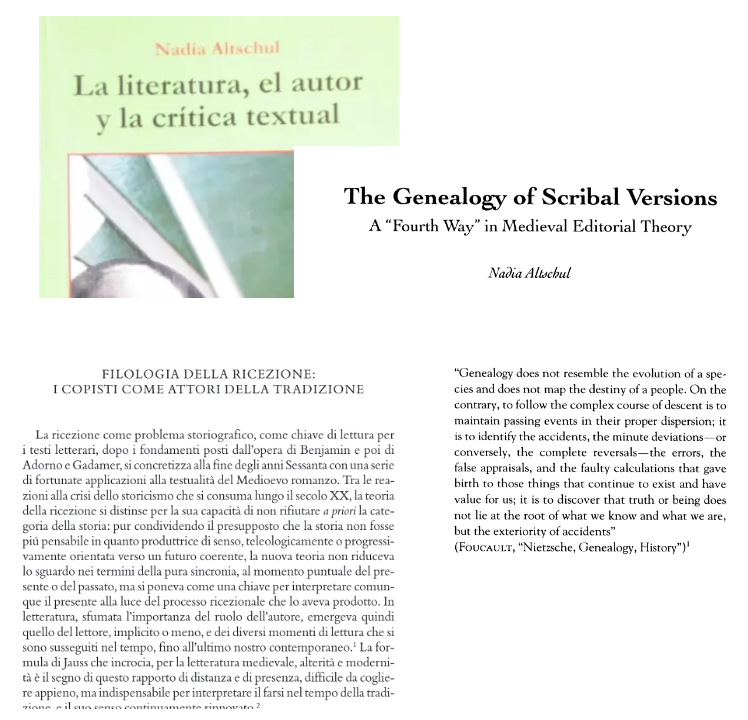
\includegraphics[width=1.2\linewidth]{img/scribal_versionism.png}
    \end{figure}
    \end{minipage}%
    \hfill
    \begin{minipage}{.45\textwidth}

    \begin{itemize}
    \item Une histoire complète des textes
    \item Stemma
    \begin{itemize}
        \item Une histoire globale des traditions textuelles
        \item Prise en compte des versions "minoritaires"
        \item Comprendre les relations entre les témoins
    \end{itemize}
    \item Ex. Nadia Altschul, Lino Leonardi (parmi d'autres)
    \end{itemize}
    \end{minipage}
    
\end{frame}



\begin{frame}{Tradition, document, texte}

    \begin{definition}
        La \textbf{tradition} (ou l'oeuvre) désigne l'ensemble des témoins manuscrits qui peuvent être rapprochée de près ou de loin d'une tradition littéraire connue. Ex. Le petit chaperon rouge. 
    \end{definition}
    
    \begin{definition}
        Le \textbf{document} désigne le support matériel qui transmet une forme particulière, tant dans sa disposition que dans son contenu, d'une tradition donnée. 
    \end{definition}
    
    \begin{definition}
        Le \textbf{texte} c'est selon les auteurs, soit le contenu textuel d'un document, soit une abstraction de ce que pourrait-être le "texte de la Genèse" ou "le texte du petit chaperon rouge". Pour certains chercheurs, le texte, dans ce sens, n'existe pas. 
    \end{definition}

\end{frame}

\begin{frame}{Auteur et scribe}

\begin{definition}
    Un \textbf{auteur} ou une \textbf{autrice} est une personne qui a mis par écrit "un texte", sur un "document" qui, par la suite, a pu donner lieu à une "tradition". Pour certain chercheurs, l'auteur n'existe pas.
\end{definition}

\begin{definition}
    Un scribe est une personne qui transmet un texte en lui apportant des modifications. En ce sens, certains chercheurs considèrent le scribe comme un des multiples auteurs du texte.
\end{definition}
    
\end{frame}




\end{document}